\chapter{Math (Probability, Statistics, Linear Algebra, etc.)}

\section{Computational Science (APMA 4302, K. Mandli) }
\subsection*{Syllabus}
\subsubsection*{Shell basics}
\subsubsection*{Version control}
\subsubsection*{Reproducibility}
\subsubsection*{Verification and validation techniques}
\subsubsection*{Shell basics}

\subsection*{}

\subsubsection*{Pillars of Science: } Experiment, Theory, Computation.


\begin{itemize}
\item
	Computation and specifically simulation has started to bring about a third pillar of science.

\item
	Experiment gives concrete basis to theory. Simulation allows us to run experiments on things that we don't have to wait to observe. Computation can tell you what experiments to run.
\end{itemize}

\begin{wrapfigure}{L}{0.5\textwidth}
	\centering
	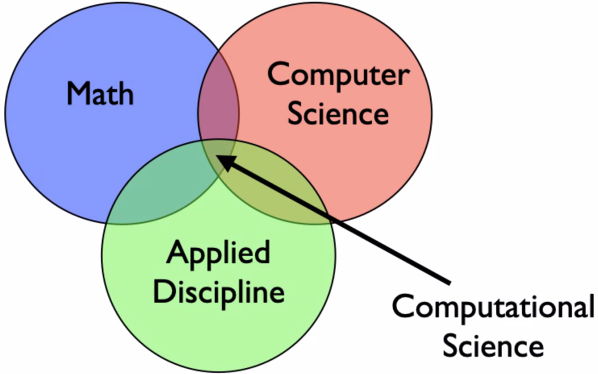
\includegraphics[width=0.7\linewidth]{images/computational_science_venn_diagram}
	\caption{}
	\label{fig:computationalsciencevenndiagram}
\end{wrapfigure}
ekekekek


